\documentclass[12pt,a4paper]{article}
\usepackage{amsmath,amscd,amsbsy,amssymb,latexsym,url,bm,amsthm}
\usepackage{epsfig,graphicx,subfigure}
\usepackage{enumitem,balance}
\usepackage{wrapfig}
\usepackage{mathrsfs,euscript}
\usepackage[usenames]{xcolor}
\usepackage{hyperref}
\usepackage[vlined,ruled,linesnumbered]{algorithm2e}
\usepackage{float}
\usepackage{cite}
\usepackage{booktabs}
\usepackage{listings}
\usepackage{xcolor}
\lstset{
    language=Python,
    basicstyle=\ttfamily,
    keywordstyle=\color{blue}\ttfamily,
    stringstyle=\color{red}\ttfamily,
    commentstyle=\color{brown}\ttfamily,
    morecomment=[l][\color{magenta}]{\#},
    numbers=left,
    numberstyle=\tiny\color{gray},
    numbersep=5pt,
    showspaces=false,
    showstringspaces=false,
    frame=single
}
\hypersetup{colorlinks=true,linkcolor=black}

\newtheorem{theorem}{Theorem}
\newtheorem{lemma}[theorem]{Lemma}
\newtheorem{proposition}[theorem]{Proposition}
\newtheorem{corollary}[theorem]{Corollary}
\newtheorem{exercise}{Exercise}
\newtheorem*{solution}{Solution}
\newtheorem{definition}{Definition}
\theoremstyle{definition}

\renewcommand{\thefootnote}{\fnsymbol{footnote}}

\newcommand{\postscript}[2]
 {\setlength{\epsfxsize}{#2\hsize}
  \centerline{\epsfbox{#1}}}

\renewcommand{\baselinestretch}{1.0}

\setlength{\oddsidemargin}{-0.365in}
\setlength{\evensidemargin}{-0.365in}
\setlength{\topmargin}{-0.3in}
\setlength{\headheight}{0in}
\setlength{\headsep}{0in}
\setlength{\textheight}{10.1in}
\setlength{\textwidth}{7in}
\makeatletter \renewenvironment{proof}[1][Proof] {\par\pushQED{\qed}\normalfont\topsep6\p@\@plus6\p@\relax\trivlist\item[\hskip\labelsep\bfseries#1\@addpunct{.}]\ignorespaces}{\popQED\endtrivlist\@endpefalse} \makeatother
\makeatletter
\renewenvironment{solution}[1][Solution] {\par\pushQED{\qed}\normalfont\topsep6\p@\@plus6\p@\relax\trivlist\item[\hskip\labelsep\bfseries#1\@addpunct{.}]\ignorespaces}{\popQED\endtrivlist\@endpefalse} \makeatother
\setlength{\parindent}{0pt}
\bibliographystyle{acm}

\begin{document}
\title{\textbf{Homework 1}}
\author{Your Name}
\date{Your Student ID}
\maketitle

\tableofcontents
\newpage

\section{Introduction}
In Deep Learning, many things matter, and thus we prepare 5 questions to cover most of them. You shall understand Network Structure, Tensor Shape, and Execution Time in \textbf{Q1}; you shall understand Back Propagation (BP) and Automatic Differentiation (AD) in \textbf{Q2}; you shall grasp Optimization Scheme in \textbf{Q3}; you shall then understand basic hyper-parameter tuning, i.e.,  Batch Size and Epoch Number in \textbf{Q4}; after understanding everything above, you are doomed to dive into On-Edge Training to understand Dataset and the challenges for on-edge learning in \textbf{Q5}. 

We sincerely hope you enjoy your journey through this homework as we do.

\section{Q1: Tensor Shape \& Execution Time (15')}
Network Definition is the biggest components of Deep Learning. In this problem, you learn how to profile tensors' shape and execution time.

\subsection{Problem Formulation}
Network for Q1:

\begin{lstlisting}[language=Python, label=network, caption=network structure]{H}
class Network(nn.Module):
    def __init__(self):
        super(Network, self).__init__()
        self.layers = []
        self.layers.append(nn.Conv2d(1, 10, kernel_size=5))
        self.layers.append(nn.ReLU(inplace=True))
        self.layers.append(nn.MaxPool2d(kernel_size=2))
        self.layers.append(nn.Conv2d(10, 20, kernel_size=5))
        self.layers.append(nn.ReLU(inplace=True))
        self.layers.append(nn.MaxPool2d(kernel_size=2))
        self.layers.append(nn.Flatten())
        self.layers.append(nn.Linear(320, 50))
        self.layers.append(nn.Linear(50, 10))
        self.layers = nn.ModuleList(self.layers)

    def forward(self, x):
        # print()
        for layer in self.layers:
            # start = time.time()
            x = layer(x)
            # end = time.time()
            # print(x.shape, "{0:d} mu s".format(int((end-start)*1e6)), sep=" ")
        return x
\end{lstlisting}

\begin{enumerate}
    \item (5') Q: Fill in Table \ref{shape+time profile}, print the shape of each layer's output. The first 2 are done for you.

    (Hint: See reference for \textit{torch.Tensor} class.

    \href{torch.Tensor}{https://pytorch.org/docs/stable/tensors.html\#torch-tensor})
    
    \item (5') Q: Fill in Table \ref{shape+time profile}, profile the execution time of each layer, both on CPU or on GPU. The first 2 are done for you. 
    
    (Hint: timing in $\mu s$)
    
\textbf{    (Hint: You shall not profile the first few batches on GPU, because GPU is warming up!!!! Also, measure multiple times on CPU, because CPU time is subject to multi-threading!!!)}
    
    \item (5') Q: Explain how to calculate the shape of the outputs of layers.
    
    (Hint: Look into the following links, learn how to compute the shape change of nn.Conv2d, nn.MaxPool2d, nn.Flatten, nn.Linear. 

    \href{nn.Conv2d}{https://pytorch.org/docs/stable/generated/torch.nn.Conv2d.html}

    \href{nn.MaxPool2d}{https://pytorch.org/docs/stable/generated/torch.nn.MaxPool2d.html}

    \href{nn.Flatten}{https://pytorch.org/docs/stable/generated/torch.nn.Flatten.html}

    \href{nn.Linear}{https://pytorch.org/docs/stable/generated/torch.nn.Linear.html})
    
\end{enumerate}

\subsection{Solution}
\begin{enumerate}
    \item (5') See Table \ref{shape+time profile}.
    \item (5') See Table \ref{shape+time profile}.
    Layer id follows what presents in Listing \ref{network}. (32 is the batch size. represent it to be N.)
    \begin{table}[H]
        \centering
        \begin{tabular}{cc|c|cc}
        \toprule[1.5pt]
            layer & type & shape of output tensor (N=32) & CPU time ($\mu s$) & GPU time ($\mu s$) \\
            \hline
            input & / & [N, 1, 28, 28] & / & / \\
            0 & Conv2d & [N, 10, 24, 24] & 1387 & 738\\
            1 & ReLU & [N, 10, 24, 24] & 3144 & 267 \\
            2 & MaxPool2d & & & \\
            3 & Conv2d & & & \\
            4 & ReLU & & & \\
            5 & MAxPool2d & & & \\
            6 & Flatten & & & \\
            7 & Linear & & & \\
            8 & Linear & & & \\
        \bottomrule[1.5pt]
        \end{tabular}
        \caption{Shape \& Time Profile}
        \label{shape+time profile}
    \end{table}
    \item (5') 
    (Your answer here !!!)
\end{enumerate}


\section{Q2: Backward Propagation (15')}
\subsection{Problem Formulation}
     (15') Q: Calculate gradient for Linear layer. 
    
    That is, you need to calculate ($\frac{\partial L}{\partial X}$, $\frac{\partial L}{\partial W}$, $\frac{\partial L}{\partial b}$), given (X, W, b, $\frac{\partial L}{\partial Y}$).

    Linear Layer Forward Algorithm is as follows:

    \begin{equation}
        Y[n,t,f] = b[f] + \sum_{c=0}^{C} X[n,t,c]\cdot W[c,f]
    \end{equation}

    Linear Layer Backward Algorithm is as follows (chain rule):

    Input: (X,W,b,$\frac{\partial L}{\partial Y}$)

    \begin{equation}
        \begin{aligned}
            &\frac{\partial L}{\partial X[n,t,c]} = 
            \sum_{f}^F\frac{\partial L}{\partial Y[n,t,f]}\cdot \frac{\partial Y[n,t,f]}{\partial X[n,t,c]}= \sum_{f}^F\frac{\partial L}{\partial Y}[n,t,f]\cdot W[c,f]\\
            &\frac{\partial L}{\partial W[c,f]} = 
            TODO \\
            &\frac{\partial L}{\partial b[f]} = 
            TODO \\
        \end{aligned}
    \end{equation}

    \textbf{    Please Calculate $\frac{\partial L}{\partial W}$ and $\frac{\partial L}{\partial b}$ yourself!!!}

    (You can learn more of PyTorch backward implementation yourself on 
    
    \href{extend}{https://pytorch.org/docs/stable/notes/extending.html\#extending-autograd})

\subsection{Solution}
    Calculate ($\frac{\partial L}{\partial X}$, $\frac{\partial L}{\partial W}$, $\frac{\partial L}{\partial b}$), given (X, W, b, $\frac{\partial L}{\partial Y}$).
    
    For example, $\frac{\partial L}{\partial X}$ is calculated for you as follows.

    \textbf{    Please Calculate $\frac{\partial L}{\partial W}$ and $\frac{\partial L}{\partial b}$ yourself!!!}

    (Your answer here!!!)
    
    Input: (X,W,b,$\frac{\partial L}{\partial Y}$)

    \begin{equation}
        \begin{aligned}
            &\frac{\partial L}{\partial X[n,t,c]} = 
            \sum_{f}^F\frac{\partial L}{\partial Y[n,t,f]}\cdot \frac{\partial Y[n,t,f]}{\partial X[n,t,c]}= \sum_{f}^F\frac{\partial L}{\partial Y}[n,t,f]\cdot W[c,f]\\
            &\frac{\partial L}{\partial W[c,f]} = 
            TODO \\
            &\frac{\partial L}{\partial b[f]} = 
            TODO \\
        \end{aligned}
    \end{equation}




\section{Q3: Optimization: Gradient Descent (15')}
\subsection{Problem Formulation}
(15') You shall implement your own optimizer class \textit{Nesterov}.

SGD with Nesterov Momentum follows the paper "A method for unconstrained convex minimization problem with the rate of convergence $O(1/k^{2})$". It has better convergence results than standard sgd. The pseudo code is as follows in Alg \ref{Nesterov}, you shall implement it in PyTorch.

\begin{center}
    \begin{minipage}[T]{0.78\textwidth}
\begin{algorithm}[H]
    \caption{Nesterov}
    \label{Nesterov}
    \KwIn{dataset: $X = \{x_1, \dots ,x_N\}$, learning rate lr, Parameters $W$, loss function $f(x_i,W)$}
    \KwOut{Best $W$}    
    initialize $W$, 2 buffers V1, V2.

    V1=V2=W, k=2
    
    \For{e=1 to E}{
        \For{i=1 to N}{
            $V2 \longleftarrow V1$
            
            $V1 \longleftarrow W - lr \cdot \nabla_W f(x_i,W)$

            $W \longleftarrow V1 + \frac{k-2}{k+1}(V1-V2)$ // V1-V2 is nesterov momentum

            $k \longleftarrow k+1$ // k is iteration counter.
        }
    }
    
    \Return{$W$}
    
\end{algorithm}
\end{minipage}
\end{center}

Compare it with the Standard Gradient Descent Scheme in Alg \ref{SGD}.

\begin{center}
    \begin{minipage}[T]{0.78\textwidth}
\begin{algorithm}[H]
    \caption{Standard SGD}
    \label{SGD}
    \KwIn{dataset: $X = \{x_1, \dots ,x_N\}$, learning rate lr, Parameters $W$, loss function $f(x_i,W)$}
    \KwOut{Best $W$}
    initialize $W$
    
    \For{e=1 to E}{
        \For{i=1 to N}{
            $W \longleftarrow W - lr \cdot \nabla_W f(x_i,W)$
        }
    }
    
    \Return{$W$}
    
\end{algorithm}
\end{minipage}
\end{center}

\subsection{Solution}
Most of code is done for you in \textit{q3code.py}. \textbf{However, you still need to implement Alg \ref{Nesterov} in \textit{step()}.}

\begin{lstlisting}[language=Python, caption=Nesterov Optimizer, label=optimizer]{H}
class Nesterov(object):
    def __init__(self, parameters, lr=1e-3) -> None:
        self.counter=2 # k
        self.lr = lr
        self.parameters=list(parameters) # W
        self.buffer1=[] # V_{k-1}
        self.buffer2=[] # V_{k-2}
        for param in self.parameters:
            tensor1 = torch.zeros_like(param.data)
            tensor2 = torch.zeros_like(param.data)
            tensor1[:] = param.data
            tensor2[:] = param.data
            self.buffer1.append(tensor1)
            self.buffer2.append(tensor2)
            self.buffer1[-1]._require_grad=False
            self.buffer2[-1]._require_grad=False
    
    def zero_grad(self):
        for param in self.parameters:
            param._grad = None
    
    def step(self):
        for param, param_m1, param_m2 in zip(
            self.parameters, self.buffer1, self.buffer2):
            # Example: SGD updates
            # param.data[:] = param.data - self.lr * param.grad
            # ##############################
            # TODO: Your code here!

            # ###############################
            None
        self.counter += 1
\end{lstlisting}

You shall install matplotlib on your nano.
\textit{sudo apt-get install python-matplotlib}

You shall reproduce my results in Figure \ref{compare-opt}, and \textbf{replace my figure with yours}.

\begin{figure}[H]
    \centering
    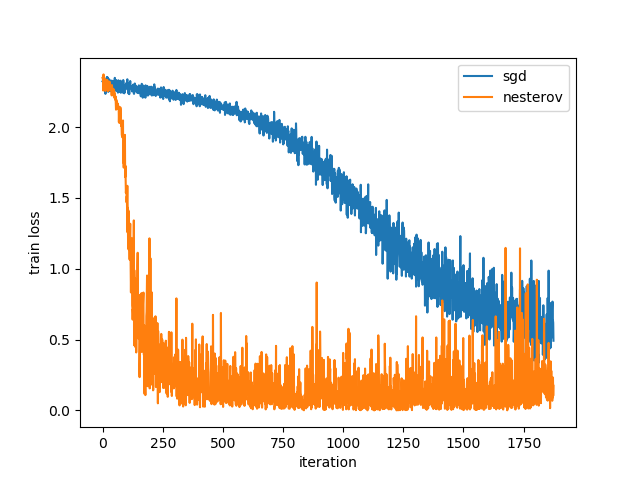
\includegraphics[width=0.7\textwidth]{optimizer.png}
    \caption{Optimizer Comparison}
    \label{compare-opt}
\end{figure}

(Your answer here!!!)

\section{Q4: Hyper-parameters: Batchsize v.s. Epoch (15')}
\subsection{Problem Formulation}

In Deep Learning training loop, there are many hyper-parameters, among which batchsize and epoch number matter most.

\begin{enumerate}
    \item (5') Fill in Table \ref{hyper-param}, to see the effect of batchsize (B) on the variance of loss $(Var[L])$. You shall also conduct experiment to visualize the results with matplotlib.
    \item (10') Fill in Table \ref{hyper-param}, to see the effect of iteration number on the mean of loss $(\mathbb{E}[L])$. You shall also conduct experiment to visualize the results with matplotlib.
    
    (\textit{Hint:} iteration number=$\frac{N}{B} \cdot E$)
\end{enumerate}

\subsection{Solution}
\begin{table}[H]
    \centering
    \begin{tabular}{c|ccc|cc}
    \toprule[1.5pt]
        expr & B & E & $\frac{N}{B} \cdot E$ & Var[L] & $\mathbb{E}[L]$ \\
        \hline
        1 & 8 & 4 & & & \\
        1 & 16 & 4 & & & \\
        1 & 32 & 4 & & & \\
        1 & 64 & 4 & & & \\
        2 & 8 & 1 & & & \\
        2 & 16 & 1 & & & \\
        2 & 32 & 1 & & & \\
        2 & 64 & 1 & & & \\
        2 & 128 & 1 & & & \\
    \bottomrule[1.5pt]
    \end{tabular}
    \caption{Hyper Parameters}
    \label{hyper-param}
\end{table}
(Your answer here !!!)
(Your figures here !!!)

\section{Q5: Have Fun on cifar100 (40')}
\subsection{Problem Formulation}
Now, it's time for you to train your own network on cifar100. You shall take care of your Dataset and DataLoader yourself. You can devise your own network to beat mine. However, you shall keep in mind that the memory upper bound for you is limited, and thus any attempts for a large model are not possible.

\begin{enumerate}
    \item (40') Finish the code, with your own model.

    \textit{(Hint:)} Remember what you have learned in Q1,2,3,4. You can adjust your network structure, optimizer, batchsize and epoch number, and even resize swap size to enlarge the memory available.
\end{enumerate}

\subsection{Solution}
(Your answer here!!!!
   Try to beat my results in Table \ref{fine-tune}. No problem if you can't.)
    \begin{table}[H]
        \centering
        \begin{tabular}{c|cc|cc}
        \toprule[1.5pt]
        & B & E & train loss & test accuracy \\
        \hline
        hzx & 4 & 10 & 4.38 & 22.1\% \\
        hzx & 4 & 50 & 3.95 & 38.0\% \\
        Yours &  &  & & \\
        \bottomrule[1.5pt]
        \end{tabular}
        \caption{Your Results}
        \label{fine-tune}
    \end{table}

\section{What have you learned?}
\subsection{Problem Formulation}
Tell TA what you have learned, and the more you learned, the more points you will earn.

\subsection{Tell me what you have learned}
(Your answer here !!!)

\section{Acknowledgement}
(Your answer here !!!)


\bibliography{ref}
\end{document}